\subsubsection{Recurrent networks}
\label{sec:theory-recurrent} 

In \emph{recurrent} neural networks also cycles of connections are allowed. In other words, the output of a particular unit could affect its input. Therefore, the activations in general could not be computed only by one forward pass. This introduces real valued dynamic systems for computing the activations. We can observe that it holds that $\partial\eta / \partial t = 0$ for the activations of neurons in the fixed point state. There are several approaches solving these dynamic systems and deriving the learning rule~\citep{pineda1987generalization, pearlmutter1989learning, williams1989learning, elman1990finding, haykin1994neural}. 

\begin{figure}[H]
  \centering
  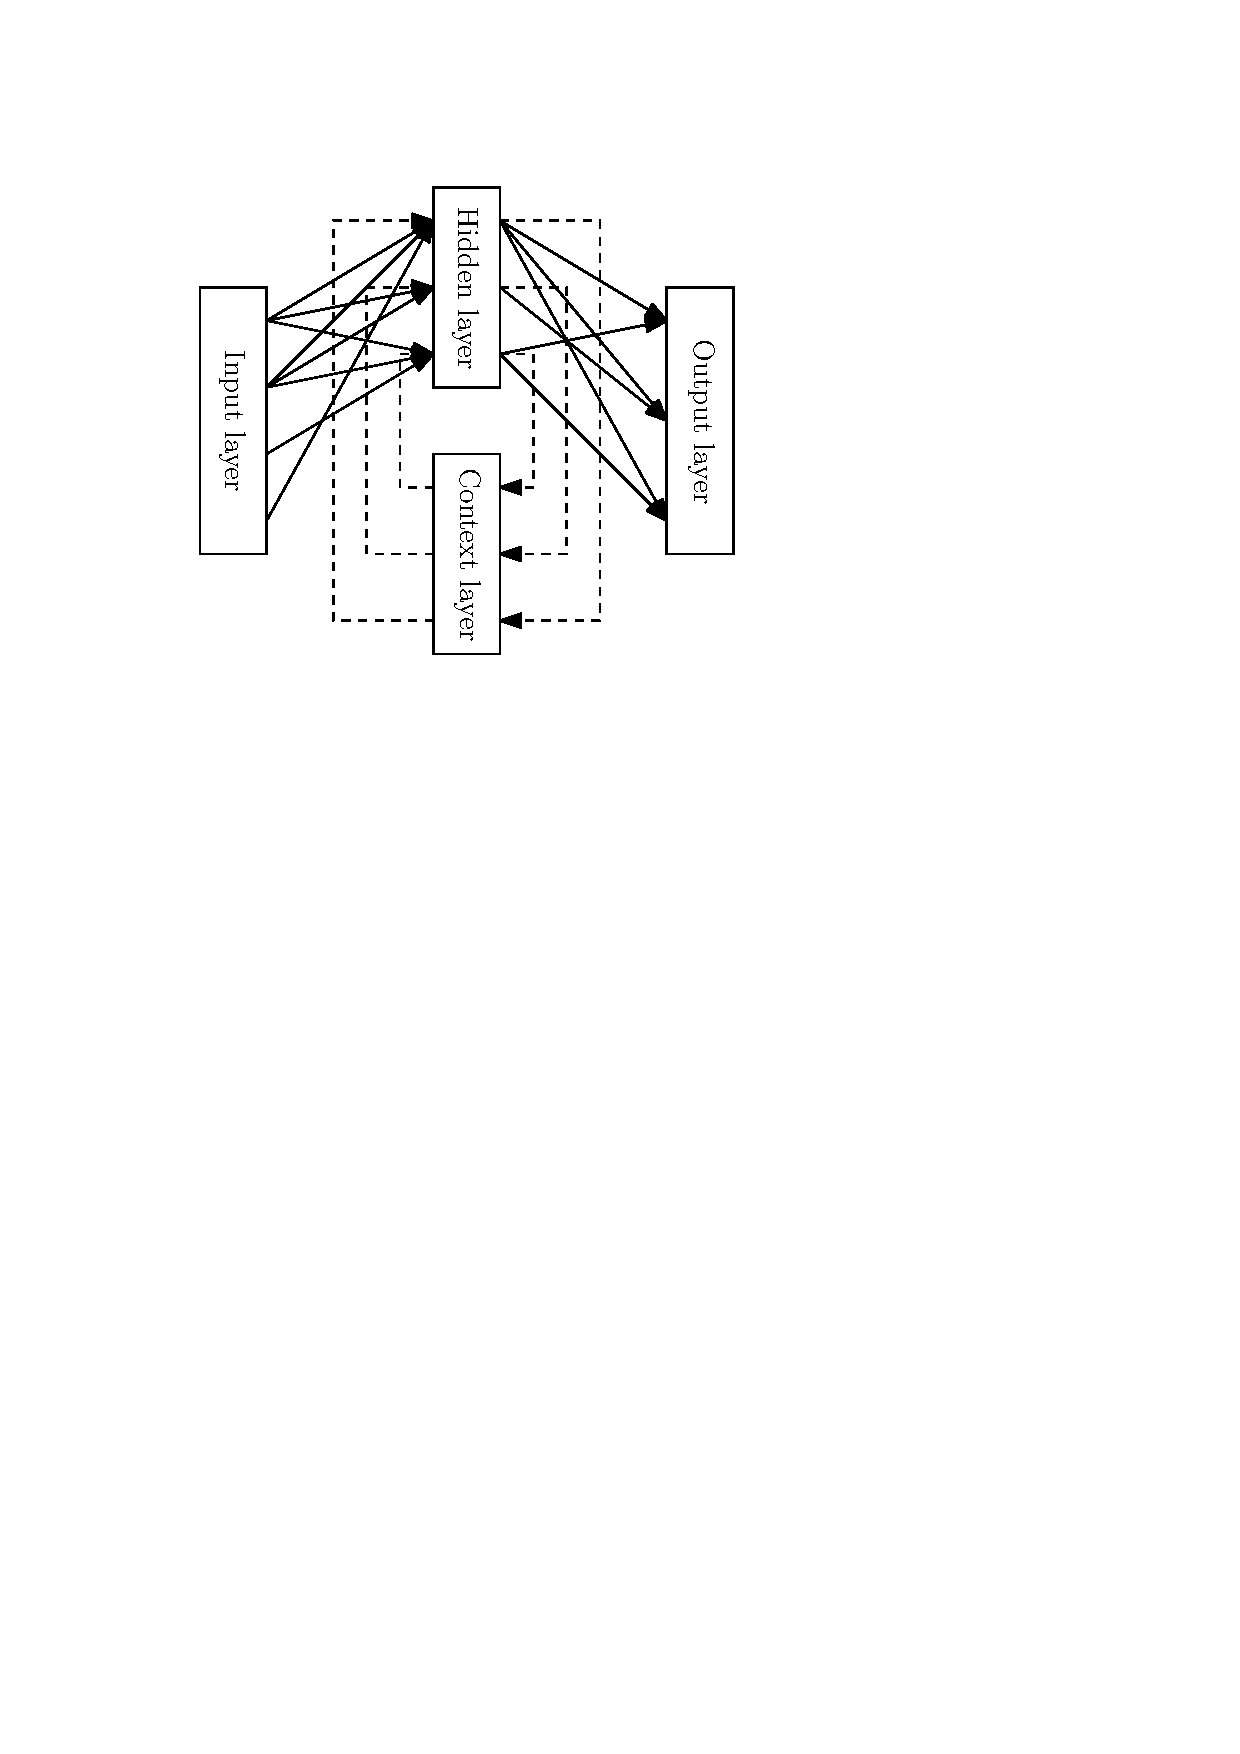
\includegraphics[width=0.4\textwidth]{img/models-recurrent.pdf}    
  \caption{Simple recurrent network proposed by~\citet{elman1990finding}. Taken from~\citet{haykin1994neural}.} 
  \label{fig:theory-recurrent}
\end{figure}

An \emph{iterative method} is used by~\citet{movellan1990contrastive} to compute activations. In the first step the input neurons have activations equal to the input vector and the other neurons have activations equal to zero. In the next steps activations from the last step are used to compute activation in the current step as shown in equation~(\ref{eq:theory-recurrent-activation}): 
\begin{equation}
  \label{eq:theory-recurrent-activation} 
  \eta_i(t+1) = \phi\left(\sum_j w_{ji}\eta_i(t)\right) 
\end{equation}
This rule is iterated while the activations are not settled. For particullar symmetric networks it can be proved that activations will converge~\citep{o1996bio}. For more general networks a dynamic system based on rule~(\ref{eq:theory-recurrent-activation}) could be introduced. The the fixed point solution is the settled activation. We experimented with the iterative method for a two way version of GeneRec in~Section~(\ref{sec:our-bal-recirc}). 

